%%%%%%%%%%%%%%%%%%%%%%%%%%%%%%%%%%%%%%%%%%%%%%%%%%%%%%%%%%%%%%%%%%%%%
% LaTeX Template: Relatório de LSD
% 
%%%%%%%%%%%%%%%%%%%%%%%%%%%%%%%%%%%%%%%%%%%%%%%%%%%%%%%%%%%%%%%%%%%%%%

\documentclass[12pt]{article}
\usepackage[portuguese]{babel}
\usepackage[a4paper]{geometry}
\usepackage{graphicx, wrapfig, subcaption, setspace, booktabs}
\usepackage[T1]{fontenc}
\usepackage[utf8]{inputenc}
\usepackage[font=small, labelfont=bf]{caption}
\usepackage{url, lipsum}
\usepackage{hyperref}
\usepackage{xcolor}
\usepackage[portuguese]{babel}
\usepackage{enumitem}
\usepackage{algorithm}
\usepackage{minted}
\onehalfspacing
   
\begin{document}
   
\begin{titlepage}
    \hspace{-3.0cm}
    
\includegraphics[scale=0.5]{logo_DEETC_cor_completo.png}\\
    Licenciatura em Engenharia Informática e de Computadores\\
    Licenciatura em Engenharia Informática, Redes e Telecomunicações\\

    \begin{center}
    \vspace{0.5cm}
    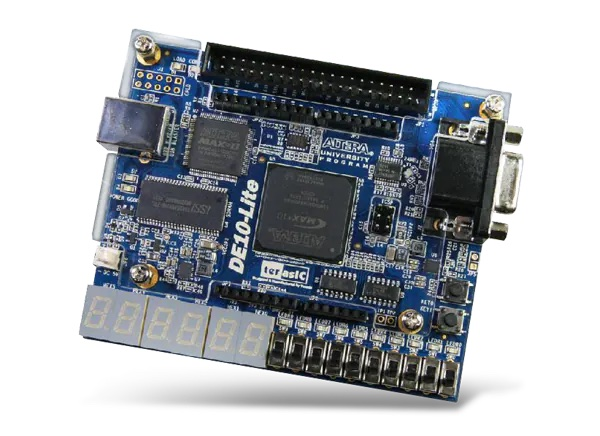
\includegraphics[width=6cm]{de10-lite.jpg}\\
    \vspace{0.5cm}

    \LARGE \uppercase{Relatório do 1$^0$ Trabalho}\\
    \textbf{Circuitos Combinatórios}
    \end{center}

    \vspace{1cm}

Trabalho realizado por:

\begin{itemize}[label={}]
    \item Número Nome
    \item Número Nome
\end{itemize}

Turma:

Docente:

\begin{center}
Lógica e Sistemas Digitais

2024 / 2025 inverno
\end{center}

\date{}

\end{titlepage}

\setcounter{page}{1}
\pagenumbering{roman} % Arabic/Indic page numbers
\addcontentsline{toc}{section}{\protect\numberline{}Índice}
\tableofcontents
\newpage

%-------------------------------------------------------------------------------
% BODY
%-------------------------------------------------------------------------------
\pagenumbering{arabic} % Arabic/Indic page numbers
\setcounter{page}{1}
\section{Objetivo}
Qual o objetivo do projeto? Qual o assunto(s) a tratar.

\section{Descrição do Circuito a Projetar}
Descrever o problema (similar ao enunciado)

\section{Desenvolvimento do Projeto}
\subsection{Funções lógicas dos circuitos}

\subsection{Simplificação lógica}


\subsection{Diagrama de blocos}


\section{Resultados e Discussão}
Explicar o que foi feito para verificar a funcionalidade do circuito. Quais os resultados obetidos

\subsection{Simulação}

\subsection{Teste}

\section{Conclusão} 
O trabalho consistiu em … \\
Foi desenvolvido em … \\ 
Foi testado na placa …\\
Os resultados experimentais confirmam o funcionamento do circuito de acordo com …


%-------------------------------------------------------------------------------
% REFERENCES
%-------------------------------------------------------------------------------
\newpage
\section*{Referências}
\addcontentsline{toc}{section}{\protect\numberline{}Referências}


\appendix
\clearpage
\section{VHDL}
\subsection{ficheiro1.vhd}
% Inserção de ficheiro de descrição hardware
\begin{minipage}{\linewidth}
\footnotesize
\inputminted{vhdl}{ficheiro1.vhd}
\end{minipage}

\subsection{ficheiro2.vhd}
% Inserção de ficheiro de descrição hardware
\begin{minipage}{\linewidth}
\footnotesize
\inputminted{vhdl}{ficheiro2.vhd}
\end{minipage}

\clearpage
\section{Esquema Elétrico}
\end{document}

%-------------------------------------------------------------------------------
% SNIPPETS
%-------------------------------------------------------------------------------

%\begin{figure}[!ht]
%	\centering
%	\includegraphics[width=0.8\textwidth]{file_name}
%	\caption{}
%	\centering
%	\label{label:file_name}
%\end{figure}


%\begin{table}[!ht]\footnotesize
%	\centering
%	\begin{tabular}{cccccc}
%	\multicolumn{2}{c} {Exemplo de tabela} & \multicolumn{4}{c} {coluna} \\
%	\multicolumn{2}{c} {} & \multicolumn{2}{c} {xpto} & \multicolumn{2}{c} {xpto} \\
%	\multicolumn{2}{c} {} & \multicolumn{2}{c} {xpto} & \multicolumn{2}{c} {xpto} \\
%	\multicolumn{2}{c} {} & \multicolumn{2}{c} {xpto} & \multicolumn{2}{c} {xpto} \\
%	\end{tabular}
%	\caption{Título da tabela.}
%	\label{label:tabela}
%\end{table}


